\documentclass{beamer}
\beamertemplatenavigationsymbolsempty
\usecolortheme{beaver}
\setbeamertemplate{blocks}[rounded=true, shadow=true]
\setbeamertemplate{footline}[page number]

\usepackage[utf8]{inputenc}
\usepackage[english]{babel}
\usepackage{amssymb,amsfonts,amsmath,mathtext}
\usepackage{graphicx}
\usepackage{subfigure}
\usepackage{tikz}
\usepackage{array}
\usepackage{multicol}
\usepackage{hyperref}
\usepackage{algorithm}
\usepackage{algpseudocode}

% Your figures are here:
\graphicspath{ {fig/} {../figures/} }

%----------------------------------------------------------------------------------------------------------
\title[Deep Reference Priors]{Deep Reference Priors: What is the best way to pretrain a model?}
\author[Y. Gao et al.]{Yansong Gao, Rahul Ramesh, Pratik Chaudhari}

\date{\footnotesize

\par\bigskip\small Presented by: Papay Ivan}
%----------------------------------------------------------------------------------------------------------
\begin{document}
%----------------------------------------------------------------------------------------------------------
\begin{frame}
\thispagestyle{empty}
\maketitle
\end{frame}
%-----------------------------------------------------------------------------------------------------

\begin{frame}{Problem Statement}

\[\hat{P}_n=\{(x_i,y_i)\}_{i=1}^n;x_i \in \mathbb{R}^d;y_i \in \{1 \dots C\} \]

\[x^n=(x_1, \dots x_n); y^n=(y_1 \dots y_n) \]

\[
w \in \mathbb{R}^p; p_w(y|x)
\]

\[
z=y|x; \pi(w) - prior
\]


\[
\pi^* = \underset{\pi}{\mathrm{argmax}} \, I_{\pi}(w; z)
\]


\end{frame}

\begin{frame}{Problem Statement}

\begin{block}{Key Question}
What is the optimal way to exploit extra data (labeled/unlabeled, from same/related tasks) to pretrain a model for a given task?
\end{block}

\begin{block}{Core Idea}
A pretrained representation can be viewed as a \textbf{Bayesian prior}. The optimal prior should allow the target task data to maximally influence the posterior.
\end{block}

\begin{block}{Formalization}
Use \textbf{Reference Priors} theory: priors that maximize mutual information between model weights and data:
\[
\pi^* = \underset{\pi}{\mathrm{argmax}} \, I_{\pi}(w; z)
\]
\end{block}

\end{frame}

\begin{frame}{Reference Priors vs Jeffreys Prior}

\begin{block}{Jeffreys Prior}
\begin{itemize}
\item Goal: \textbf{Reparameterization invariance}
\item Defined via Fisher Information Matrix: $\pi_J(w) \propto \sqrt{\det g(w)}$
\item \textbf{Independent} of sample size $n$
\item Always \textbf{continuous}
\end{itemize}
\end{block}

\begin{block}{Reference Prior}
\begin{itemize}
\item Goal: \textbf{Maximize data influence} on posterior
\item Maximizes mutual information: $\pi^* = \arg\max I_{\pi}(w; z)$
\item \textbf{Depends} on sample size $n$ (adaptive)
\item \textbf{Discrete} for finite $n$ (supported on atoms)
\end{itemize}
\end{block}

\end{frame}

\begin{frame}{Reference priors}

In fact we want to maximize $KL(p(w|z) | \pi(w))$

\space 


$
\pi^*=argmax_{\pi} I_{\pi}(w;z)=\int p(z) p(w|z) log[\frac{p(w|z)}{\pi(w)}] dz dw = H(w) - H(w|z)
$

Where $p(z)=\int \pi(w) p(z|w) dw$ and $H(w)=-\mathbb{E}_w [log \pi(w)]$

It is difficult to compute reference prior straight-through so we asume that
$\pi_n^*=argmax_{\pi} I (w;z^n)=H(w)-H(w|z)$

\[
lim_{n \rightarrow \infty} \pi_n^* = \pi^*
\]

NOTE!  reference prior does not exist if $I_\pi(w; z^
n)$ is infinite


\end{frame}


\begin{frame}{Blahut-Arimoto Algorithm}

\begin{block}{Iterations}

\[
\pi^{t+1}(w) \propto exp(KL(p(z|w)|p(z))) \pi^t(w)
\]
\end{block}

\begin{block}{Dependence on Sample Size}
\begin{itemize}
\item Small $n$: Prior concentrates on few diverse models
\item Large $n$: Prior converges to Jeffreys prior
\item Enables adaptation to data scarcity
\end{itemize}
\end{block}



\end{frame}

\begin{frame}
    \begin{figure}
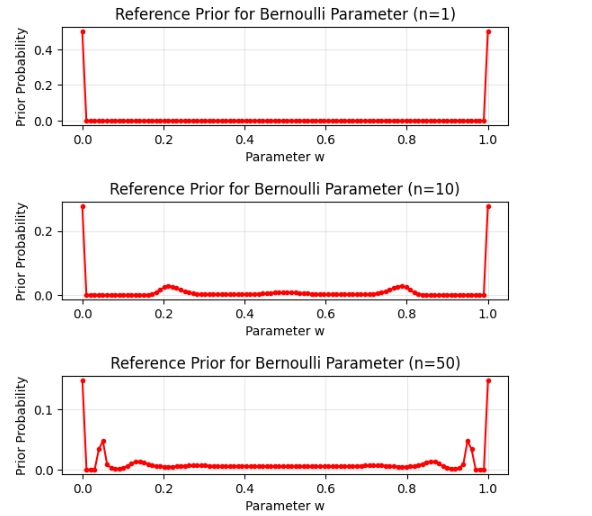
\includegraphics[width=0.7\textwidth]{coin_prior.jpg}
\caption{Reference prior for coin-tossing (n=1,10,50)}
\end{figure}
\end{frame}

\begin{frame}{Computing Reference Priors for Deep Networks}

\begin{block}{Blahut-Arimoto Algorithm with Particles}
\begin{itemize}
\item Represent prior as set of particles: $\{w^1, \ldots, w^K\}$
\item Each particle is a neural network
\item Gradient of mutual information flows to all particles
\item Particles become diverse in prediction space
\end{itemize}
\end{block}


\begin{figure}
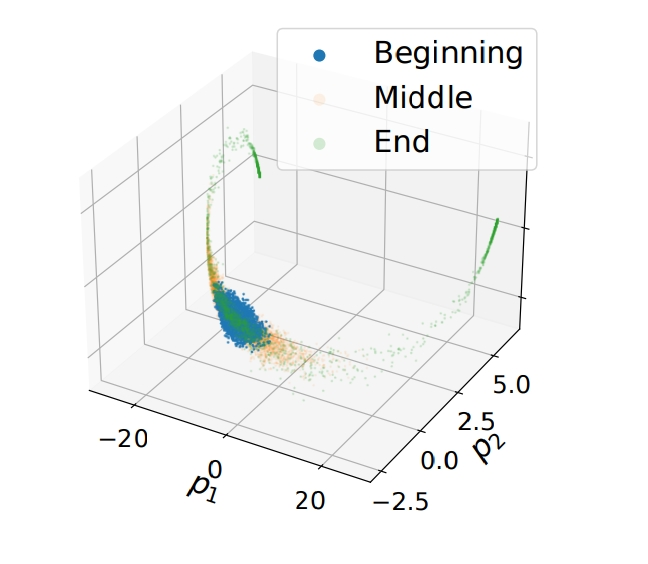
\includegraphics[width=0.5\textwidth]{particle_evolution.jpg}
\caption{Particle evolution in prediction space (MNIST 3vs5)}
\end{figure}


\end{frame}

\begin{frame}{Application 1: Semi-Supervised Learning}

\begin{block}{Formalization}
Use unlabeled data $x^u$ to build optimal prior $\pi^*(w)$:
\[
\max_{\pi} \gamma I_{\pi}(w; y^u, x^u) + \mathbb{E}_{w \sim \pi} [\log p(y^n | x^n, w)]
\]
\end{block}

\begin{block}{Connection to Practice}
\begin{itemize}
\item Explains \textbf{consistency regularization} (FixMatch)
\item Explains \textbf{entropy minimization} techniques
\item Provides theoretical foundation for SSL
\end{itemize}
\end{block}

\begin{block}{Practical Implementation}
\begin{itemize}
\item Heavy data augmentation (RandAugment, CTAugment)
\item Jensen's inequality bound for entropy computation
\item Pseudo-labeling with confidence threshold
\end{itemize}
\end{block}

\end{frame}

\begin{frame}{Application 2: Transfer Learning}

\begin{block}{Two-Stage Experiment}
\begin{itemize}
\item Stage 1: Source task data $(x_s^m, y_s^m)$
\item Stage 2: Target task data $(x_t^n, y_t^n)$
\item Goal: Optimal prior for target task
\end{itemize}
\end{block}

\begin{block}{Optimal Prior Formula}
\[
\pi_{n|m}^\beta(w) \propto \pi_n^*(w) \cdot p(y_s^m | x_s^m, w)^{-\beta}
\]
\begin{itemize}
\item $\beta = 1$: Forget source task (different tasks)
\item $\beta = 0$: Remember source task (similar tasks)
\item Connects to \textbf{Predictive Information Bottleneck}
\end{itemize}
\end{block}

\end{frame}

\begin{frame}{Experimental Results: Semi-Supervised Learning}

\begin{table}[h]
\centering
\textbf{CIFAR-10 Classification Accuracy (\%)}
\begin{tabular}{|l|c|c|c|c|c|}
\hline
Method & 50 samples  & 250 samples & 500 samples  \\
\hline
FixMatch (RA) & 86.19  & 94.93 & 93.91  \\
FlexMatch & 95.03  & 95.02 & -  \\
\textbf{Deep Reference Prior} & \textbf{85.45} &  \textbf{92.13} & \textbf{92.94}  \\
\hline
\end{tabular}
\end{table}

\begin{block}{Key Findings}
\begin{itemize}
\item Competitive with state-of-the-art methods
\item Particularly effective with very few labeled samples (5 per class)
\item Provides theoretical explanation for empirical successes
\end{itemize}
\end{block}

\end{frame}

\begin{frame}{Experimental Results: Transfer Learning}

\begin{block}{Setup}
\begin{itemize}
\item CIFAR-100, 20 five-way classification tasks
\item Source: 1000 labeled samples
\item Target: 100 labeled samples + unlabeled data
\end{itemize}
\end{block}

\begin{block}{Results}
\begin{itemize}
\item \textbf{Outperforms fine-tuning} in low-data regime
\item Effectively leverages both source labels and target unlabeled data
\item Adaptive to task relatedness via $\beta$ parameter
\end{itemize}
\end{block}

\begin{figure}
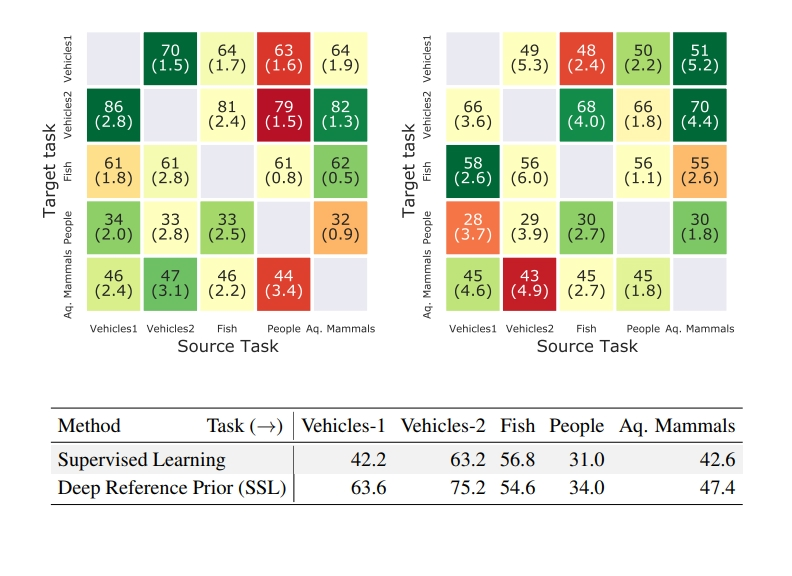
\includegraphics[width=0.5\textwidth]{transfer_results.jpg}
\caption{Transfer learning accuracy comparison}
\end{figure}

\end{frame}



\begin{frame}{Conclusions}


\begin{itemize}
\item possible to use in deep neural networks

\item maintains the reparametrization invariance of Jeffreys prior

\item helps if the number of samples
from the task available to the learner is finite

\item uses sample size while Jeffrey's prior doesn't do it
\end{itemize}

\end{frame}



\end{document}